\documentclass[11pt]{amsart}

% Standard letter size paper with 1inch margins
\usepackage[letterpaper, margin=1in]{geometry}

% Useful packages 
\usepackage{amsmath, amssymb, amsthm, amsaddr}
\usepackage{enumerate, subcaption, graphicx, hyperref}
\usepackage{xcolor}

\usepackage{algorithm}
\usepackage{algpseudocodex}

\newcommand{\reals}{\mathbb{R}}
\newcommand{\tr}{\top}
\renewcommand{\vec}[1]{\mathbf{#1}}
\newcommand{\todo}[1]{\textcolor{red}{TODO: #1}}

\DeclareMathOperator{\tf}{tf}
\DeclareMathOperator{\idf}{idf}
\DeclareMathOperator{\tfidf}{tfidf}
\DeclareMathOperator*{\argmin}{arg\,min}

\graphicspath{./res/}

\title{Fun with Flags!}
\author{Jonathan Elsner} % first and last name

\address{Department of Applied Mathematics, University of Washington, Seattle, WA 
\\ \texttt{jeelsner@uw.edu}}

\date{\today} % you can also just type the date instead of "\today"

\begin{document}

\begin{abstract}
    Flags are an important symbol of a nation, putting its values and heritage
    on display for the world. As such, it is important that a flag be well
    designed and distinctive. We use data analysis to examine similarities and
    differences between national flags to identify patterns in flag design.
\end{abstract}

\maketitle 

\section{Introduction and Overview}\label{sec:Introduction}

Flags are important national symbols. A well-designed flag can be a source of
pride for the citizens of a country, and contribute to a country's brand across
the world. Famous flags are instantly identifiable and immediately invoke
powerful emotions and ideals, becoming metonymic for the country and principles
they stand for, like the association of the flag of the United States with
freedom and equality. The best flags are simple and unique, easily identifiable
far away on a flagpole or across a handshake on a lapel pin.

According to ``Good'' Flag, ``Bad'' Flag from the North American
Vexillological\footnote{Vexillology is the study of the history, symbolism, usage,
and design of flags.} Association \cite{good-flag-bad-flag}, there are five
basic principles of flag design:
\begin{enumerate}
    \item Keep it simple: The flag should be so simple that a child can draw it
    from memory.
    \item Use meaningful symbolism: The flag's images, colors, or patterns
    should relate to what it symbolizes.
    \item Use two to three basic colors: Limit the number of colors of the flag
    to three, which contrast well and come from the standard color set.
    \item No lettering or seals: Never use writing of any kind or an
    organization's seal.
    \item Be distinctive or be related: Avoid duplicating other flags, but use
    similarities to show connections.
\end{enumerate}

Obviously, these are merely guidelines, and as flags are the product of cultural
and political processes, rarely adhered to. For example, the flags of Chad and
Romania (see Figure \ref{fig:chad-romania}) completely fail tenet five (be
distinctive or be related) as the countries are completely politically and
culturally unrelated while their flags are extremely similar.

\begin{figure}[h!]
    \centering
    
\includegraphics[width=0.5\textwidth]{./res/left_chad_right_romania.png}
    \caption{Two confusing flags. The flag of Chad on the left and the flag of
    Romania on the right. These flags are identical except for the shade of
    blue: Chad's is indigo (hex \texttt{\#00205B}), while Romania is simply blue (hex
    \texttt{\#012169}). The similarity of these flags has caused minor international
    conflict, with Romania refusing to consider changing the flag in 2004 after
    unconfirmed reports that Chad asked the UN to investigate the issue
    \cite{bbc-identical-flag}. \label{fig:chad-romania}}
\end{figure}

In this paper we use data analysis techniques such as PCA, \(k\)-means, and
Gaussian Mixture Models to compare and contrast descriptions of national flags
of all 193 UN member states, two observer states, and nine \emph{de facto}
states (213 flags total). Our goal is to identify groups of similar flags and
patterns within them, and highlight unique flags that are exemplary of the five
rules listed above. We hope to bring a level of objectivity to this task through
data analysis otherwise not present in a manual comparison of flags, although we
note the limitations of unsupervised learning methods like k-means: picking
clusters is a subjective assessment, with no objective measurement of quality
since the samples are unlabeled.
% \todo{that last sentence could be phrased better}

% Before we begin, one final note: the relationship between flags and countries is
% subtle. One nation may have multiple flags. For example, Austria has both a
% civil flag for use by citizens of the country, and a state flag, for use by
% government organizations. Perhaps more surprising is that the same national flag
% can be used by multiple countries: One of Transnistria's\footnote{Transnistria
% is an unrecognized breakaway state from Moldova with ties to Russia.} two
% national flags is the Russian National Flag, although with different
% proportions. For these reasons, in the data analysis, the flag-nation pair will
% be considered, as opposed to simply the flag. However, since in the vast
% majority of cases, the relationship between flags and countries is one-to-one,
% for concision we will only refer to the name of the flag, unless it is otherwise
% unclear.
% \todo{flags of Russia and Transnistria figure?}

\section{Theoretical Background}\label{sec:theory}

\subsection*{Term Frequency-Inverse Document Frequency (tf-idf)}

Term frequency-inverse document frequency (tf-idf) is a measure of the
importance of a word present in a document out of a larger corpus of documents.
It comprises two parts: term frequency, and inverse document frequency.

Term frequency (tf) is the
number of times a word is present in a given document. This characterizes how
important the word is within a document. Generally, a word that shows up many
times in a document is important. Term frequency is computed by
\[ \tf(t, d) = \frac{c_{t, d}}{\sum_{t' \in d} c_{t', d}}\]
where \(t\) is the
term in question, \(d\) is the document in question, and \(c_{t, d}\) is the
number of times (i.e. \emph{\textbf{c}}ount) term \(t\) occurs in document \(d\).

Inverse document frequency (idf) measures how important a word is overall.
Intuitively, common words like `the' and `to' do not give very much context to
any specific document because they have no meaning specific to a topic. So even
though they occur frequently and consequently have a high \(\tf\), they should
be weighted lower. Inverse document frequency achieves this by measuring how
often a term appears in the entire corpus of documents. \(\idf\) is computed as
follows:
\[ \idf(t, D) = \log \frac{|D|}{|\left\{ d : d \in D \text{ and } t \in
d\right\}|}\] where \(D\) is the set of all documents \(d\) (the ``corpus'').
This quantity is large for rare words and small for common words.

Finally, tf-idf combines these two factors by multiplication:
\[ \tfidf(t, d, D)  = \tf(t, d) \cdot \idf(t, D) \]

\subsection*{Singular Value Decomposition (PCA)}

For any matrix \(A \in \reals^{m\times n}\), there exist unitary matrices \(U
\in \reals^{m \times m}\)
and \(V \in \reals^{n \times n}\) and a diagonal matrix \(\Sigma \in \reals^{m
\times n}\) such that
\[ A = U \Sigma V^\tr \]
where the first \(r = \text{Rank}(A)\) entries of \(\Sigma\) are called the
singular values, and the remaining entries are 0. Note that the singular values
are ordered from largest to smallest. The columns of \(U\) are
called the left singular vectors, and the columns of \(V\) are called the right
singular values.

From this we can compute the principle component analysis of a dataset. Suppose
\(X\) is a matrix whose columns are records of data collected, and each row
represents a different feature in the data. First we need to compute the average
column
\[ \bar{\vec{x}} = \frac{1}{n} \sum_{j=1}^n \vec x_j\]
and subtract it from the data matrix to get a centered version of the data
matrix:
\[ \bar X = X - \vec 1_n^\tr \vec x\]
where \(\vec 1_n\) is a vector of ones with length \(n\).
Let \(\bar X\) have PCA \(\bar X = U \Sigma V^\top\). Then, we can compute the
covariance matrix as such:
\begin{align*}
    C &= \bar X \bar X^\tr \\
      &= (U \Sigma V^\tr) (U \Sigma V^\tr)^\tr \\
      &= U \Sigma V^\tr V \Sigma U^\tr \\
      &= U \Sigma^2 U^\tr
\end{align*}

This can be interpreted as a description of the directions of the largest
variance and by how much each direction varies. In this case, The elements
\(\sigma^2\) of \(\Sigma ^2\) describe the variance in each direction, and the
corresponding vector in \(U\) is the direction of the variance. We call
these vectors principle component (PC) modes. This forms the basis of Principle
Component Analysis.

The first several PCs usually explain a large majority of the variance in the
data, and we can ignore higher-order PCs. Hence, we can project the data into a
reduced PC space and retain much of the information in the data. This is a
common data-analysis technique, because latent patterns in the data may be
revealed in PC space.

We can project a vector \(\vec x^\tr\) of data into PC space by multiplying by
\(U^\tr\) (the change-of-basis matrix into PC space):
\[ \vec x' =  U^\tr \vec x \]
if we want to reduce the dimensionality to \(k\) dimensions or PC modes, we can
truncate \(U\) by setting all columns after the \(k\)\textsuperscript{th} column
to zero. Then \(\vec x' \in \reals^k\).

Returning to the variance of the data, we can measure the size of the overall
variance using the Frobenius norm:
\[ ||X||_F = ||\Sigma||_F = \left(\sum_{i=1}^r \sigma_i^2 \right)^{1/2}\]
since the Frobenius norm is preserved for unitary matrices. Another term for
this value is the energy of the matrix \(X\). When we truncate to only a few PC
modes, we lose some of the variance or energy in the data. It is useful to
understand this loss by taking the ratio of the energy of the reduced space to
the energy of the original:
\[ \sqrt{ \frac{ \sum_{i=1}^k \sigma_i^2 }{ \sum_{i=1}^r \sigma_i^2 } } \]
where \(r\) is the rank of \(X\). Note this is equivalent to the Frobenius norm
of the matrix \(X\) approximated in \(k\) PC modes divided by the Frobenius norm
of the original matrix \cite{elsner-hw2}.
% \todo{Maybe don't self-plagarize and just copy-paste from HW 2.}


\subsection*{\(k\)-means Clustering}\label{sec:k-means}

\(k\)-means clustering is an unsupervised dimension reduction technique. The
algorithm works by creating a set of \(k\) clusters of similar samples close to
the mean of each cluster. The mean of each cluster represents a prototypical
point in the cluster. Optimal clusters minimize the variance between points in
the cluster; doing so is NP hard, so most algorithms find an approximate
solution occupying a local minimum. The most common algorithm used is ``Lloyd's
Algorithm'', described in Algorithm \ref{alg:k-means}. The initialization of the
centers before they are iteratively refined is important; poorly chosen initial
centers can result in poor clustering. The initialization in Algorithm
\ref{alg:k-means} is k-means++, which attempts to select random centers that are
far from each other.

Since \(k\)-means is an unsupervised technique, there are no labels for the
data, and therefore no optimal assignment of clusters. Deciding what clustering
is `best' is inherently subjective. The data analyst must decide whether the
clusters are well-separated and homogenous. Heuristics, such as Silhouette Score
described in section \ref{sec:silhouette-score} are helpful. Because of the
randomness in initialization, it is common to run \(k\)-means multiple times and
select the run with the `best' clustering.

The clusters created by \(k\)-means is readily visualized, creating a Voronoi
diagram.

\begin{algorithm}[!ht]
\caption{k-means}\label{alg:k-means}
\begin{algorithmic}
    \Procedure{kmeans}{k, points}
    \State \(centers_0 \gets \Call{init}{k, points}\)
    \State \(\varepsilon \gets 10^{-6}\) \Comment{Tolerance for convergence}
    \State \(d \gets False\) \Comment{Boolean tracking convergence}
    \State \(i \gets 0\) \Comment{Keep track of number of iterations}
    \While{\(\neg d\)}
        \State Create array \(clusters\) of points belonging to each cluster.
        \For{\(p \in points\)}
            \State \(a \gets \argmin_{c \in centers_i} ||p - c||\) \Comment{Assign point \(p\) to center \(a\)}
            \State Assign point \(p\) to the cluster belonging to center \(a\).
        \EndFor
        \State Take the mean of each cluster in \(clusters\) to get \(k\) new centers \(centers_{i+1}\)
        \State \(d \gets ||centers_{i+1} - centers_{i}|| < \varepsilon\)
        
    \EndWhile
    \Return \(centers, clusters\)
    \EndProcedure

    \Procedure{init}{k, points}
        \State \Comment{k-means++ is described here. Other initialization methods are possible.}
        \State Choose the first center \(c\) uniformly at random. Add it to the list of centers \(centers\).
        \While{\(|centers| < k\)}
        \State Compute the distance from nearest center already chosen to each point:
        \Statex \(d_p \gets \argmin{p\in points, c\in centers}||p - c||\)
        \State Choose an unselected point randomly proportional to \(d_p^2\) to be the next center.
        \EndWhile
        \Return \(centers\)
    \EndProcedure
\end{algorithmic}
\end{algorithm}

\subsection*{Gaussian Mixture Models (GMMs)} \label{sec:gmms}

\(k\)-means is not without its drawbacks. Most importantly, it assumes that
latent clusters contain about the same number of points and have the same
variance. If latent clusters in the data do not have uniform density,
\(k\)-means can create clusters that do not describe the data well. Gaussian
Mixture Models do not share these assumptions, and can perform better in such
cases. GMMs model clusters and the normally-distributed probability that a point
belongs to a cluster. The Expectation Maximization algorithm used to compute
these clusters is described in Algorithm \ref{alg:gmm}.

\begin{algorithm}
    \caption{Expectation Maximization for GMMs}\label{alg:gmm}
    \begin{algorithmic}[1]
        \State Initialize means \(\mu_k\), covariances \(\Sigma_k\) and mixing coefficients \(\pi_k\) and evaluate the initial value of the log likelihood.
        \State Evaluate the responsibilities using the current parameter values
        \[ \gamma(z_{n,k}) = \frac{\pi_k \mathcal{N}(x_n | \mu_k \Sigma_k)}{\sum_{j=1}^K \pi_j \mathcal{N}(x_n | \mu_j \Sigma_j)}\]
        \State Re-estimate the parameters using the current responsibilities
        \begin{align*}
            \mu_k' &= \frac{1}{N_k} \sum_{n=1}^N \gamma(z_{n, k})x_n \\
            \Sigma_k' &= \frac{1}{N_k} \sum_{n=1}^{N} \gamma(z_{n, k})(x_n - \mu_k')(x_n - \mu_k')^T \\
            \pi_k' &= \frac{N_k}{N}
        \end{align*}
        where \(N_k = \sum_{n=1}^N \gamma(z_{n, k})\)
        \State Evaluate the log likelihood
        \[ \ln p(X | \mu, \Sigma, \pi) = \sum_{n=1}^N \ln \left[\sum_{k=1}^K \pi_k \mathcal{N}(x_n | \mu_k, \Sigma_k)\right] \]
        and check for convergence of either the parameters or the log likelihood. If the convergence criterion is not satisfied return to step 2. \Comment{From \cite{bishop}.}
    \end{algorithmic}
\end{algorithm}

\subsection*{Silhouette Score}\label{sec:silhouette-score}

Heuristics exist to characterize the
effectiveness of clustering. One such metric is the Silhouette score, calculated
per point as
\[ s = \frac{b - a}{\max(a, b)} \] where \(a\) is the average distance between
the point and all other points in its cluster, and \(b\) is the average distance
between the point and all points in the next nearest cluster. The Silhouette
score for a set of data is the average of the per-sample score. This score
ranges between -1 and 1, with a score of -1 indicating a complete failure to
create clusters, and 1 indicating strong clustering \cite{sklearn-clustering}. 

\section{Algorithm Implementation and Development}\label{sec:algorithms}

% \todo{algorithms}

As a starting point for our technical analysis, we need data about the
appearance of each flag. Since it is difficult to extract meaningful and
interpretable features from images easily, we instead begin with text
descriptions of each flag supplied to us by the editors of the
\href{https://en.wikipedia.org/wiki/List_of_national_flags_of_sovereign_states}{\emph{List
of national flags of sovereign states}} Wikipedia Page \cite{list-of-flags}. We
process this text description into a tf-idf table and perform PCA on this table
to reduce the dimensionality. This approach is not without it's downsides. For
example, in the caption of Figure \ref{fig:uganda} we are given a description of
the flag of Uganda which states that the flag shows a ``grey crowned crane''. It
is not immediately obvious what a grey crowned crane looks like, so one cannot
get a complete picture of the flag. More importantly for our data analysis, this
flag description is likely the only one with the words ``grey crowned crane'' in
it, making them a dead giveaway for the flag of Uganda. However in general the
descriptions give a first approximation for the flag appearance and use similar
words to describe multiple flags.

Creating the tf-idf table, we end up with 577 words describing all 213 flags.

% \todo{tf-idf table?}

Because we have more features than flags, we must use dimension reduction to
remove features that do not contribute meaningful information to the description
of the flags. Performing PCA on the tf-idf table, we found that 138 of the 213
total principal components described 99\% of the variance present in the data. 

We experimented with the optimal number of PCA dimensions to keep. We examined
clusters resulting from two, three, five, ten, twenty, fifty, 100, and 138 PCs.
Since we can readily plot two dimensions in PC-space, using two dimensions as
the input to \(k\)-means or the GMM produced the most comprehensible clusters
when visualized. However, different numbers of PCs produced better clusters.
% \todo{analyze}.

We tried \(k\)-means with values of \(k\) between three and thirty.
We then tried to use \(k\)-means to cluster similar flags, however when we
visualized the data we found that different clusters had different variances,
and \(k\)-means produced poor clusters. For this reason we switched to GMMs.

We tried GMMs with between two and thirty gaussian components for each number of
PCs listed above. Ultimately we went with a model that formed five Gaussians
with an input of two principal components. While its Silhouette Score of 0.024
was lower than other models we fit, many of those models grouped the vast
majority of flags into one category, with the remaining categories containing
only one or two outliers. The model we chose effectively striates the flags into
several categories, and the two dimensions of PCs gives it the added bonus of
being easily visualized.

\begin{figure}[!ht]
    \centering
    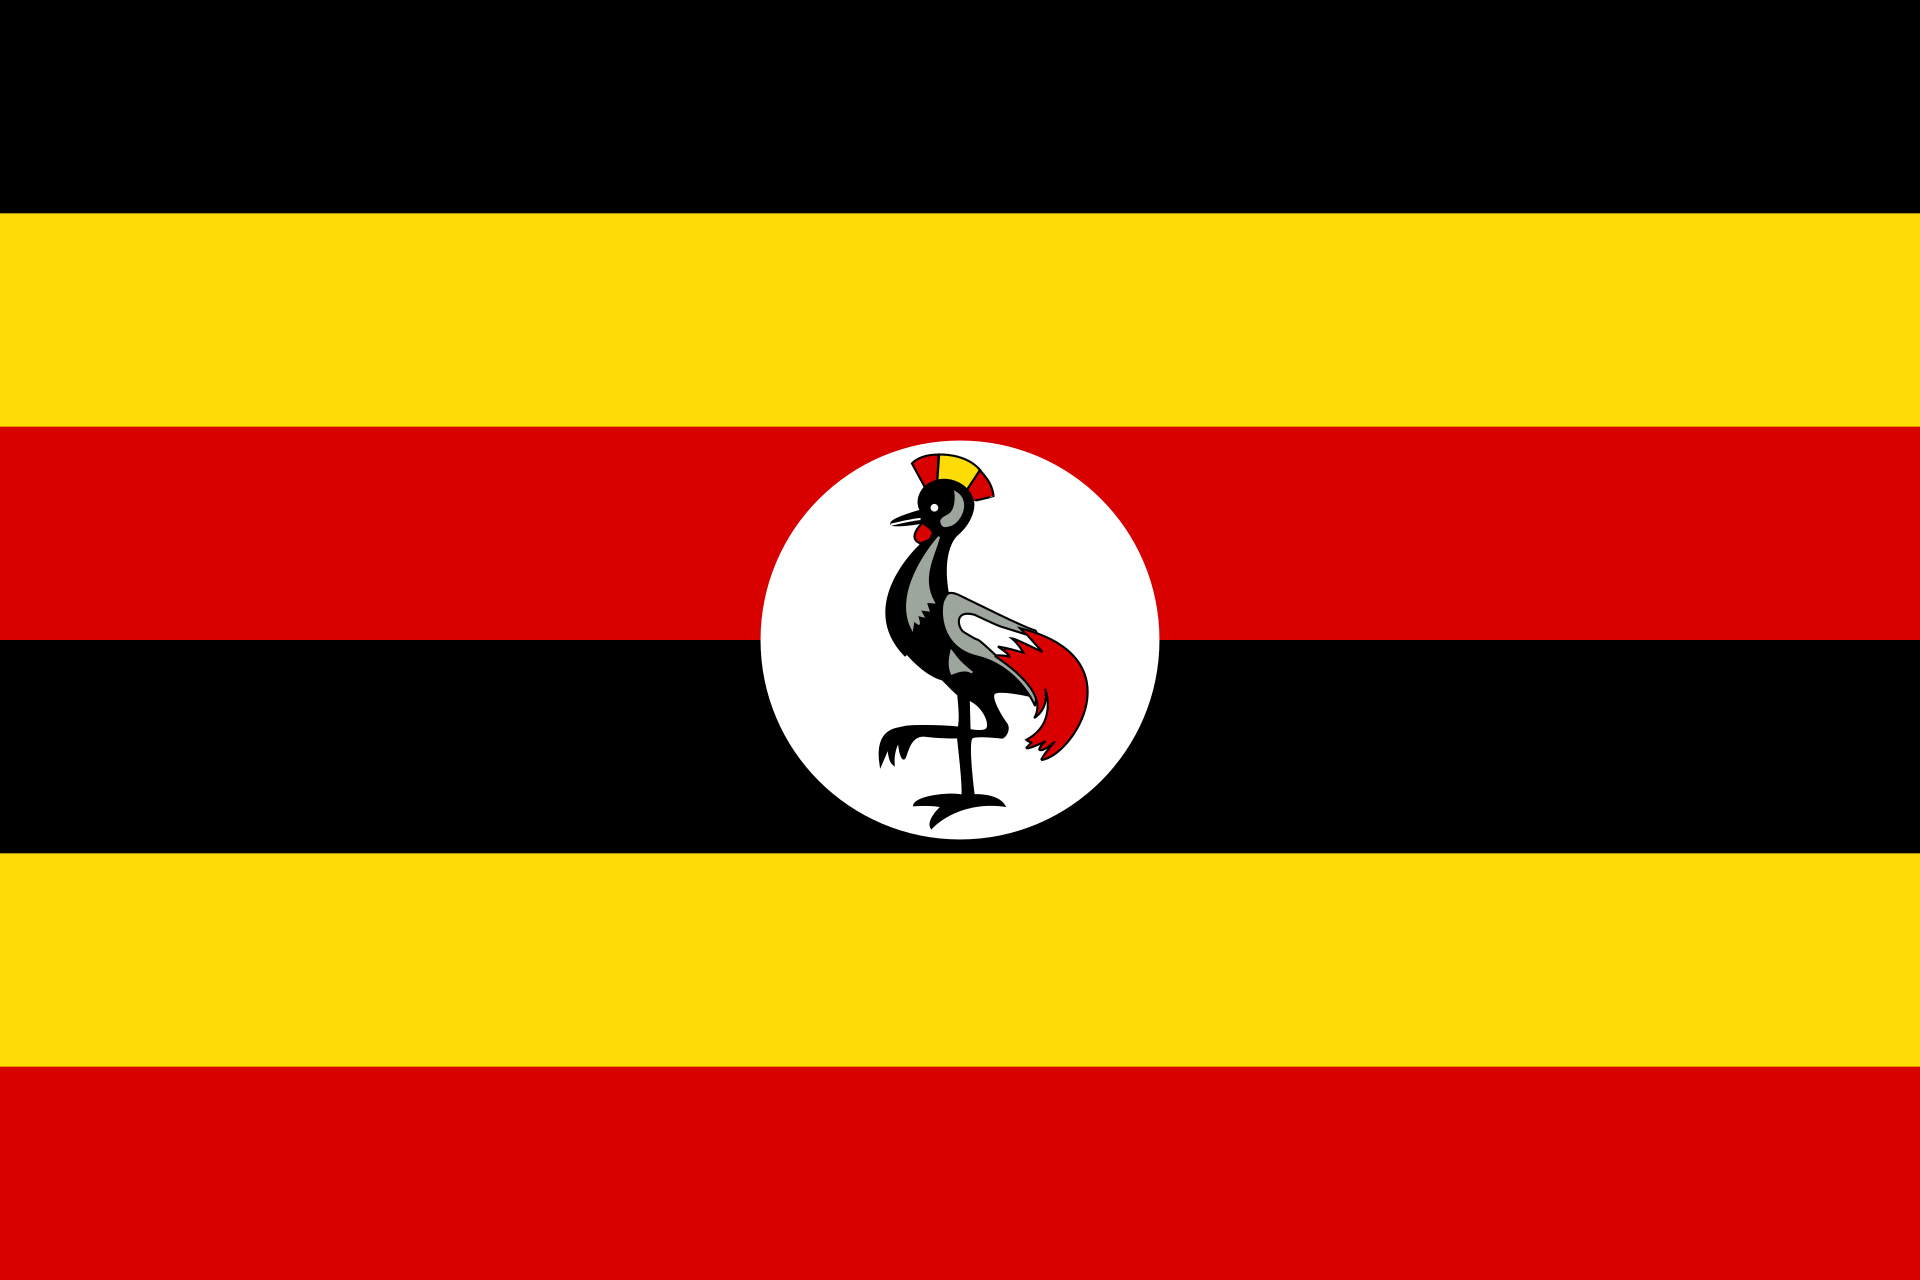
\includegraphics[width=0.25\textwidth]{./res/Flag_of_Uganda.svg.png}
    \caption{Flag of Uganda. Description on Wikipedia: \emph{Six equal
    horizontal bands of black (top), yellow, red, black, yellow, and red; a
    white disk is superimposed at the center and depicts a grey crowned crane
    (the national symbol) facing the hoist side. } \label{fig:uganda}}
\end{figure}

\section{Computational Results}\label{sec:results}

Analyzing figure \ref{fig:flag-pca}, we can readily make a few observations.
First, the first two PCs nicely separate flags with crosses in the lower
right-hand corner; Denmark, Sweden, Switzerland, and others are tightly grouped
there. Further, crosses with eight arms are nearby (the United Kingdom and North
Macedonia\footnote{North Macedonia (yellow rays on a red background)'s proximity
is especially impressive since it's description does not include the word
`cross'.}). We also see that flags with a solid circle in the middle (Japan,
Bangladesh, Palau) have also been nicely separated from other flags in the upper
right, although they are not as tightly grouped. 

\begin{figure}[!ht]
    \centering
    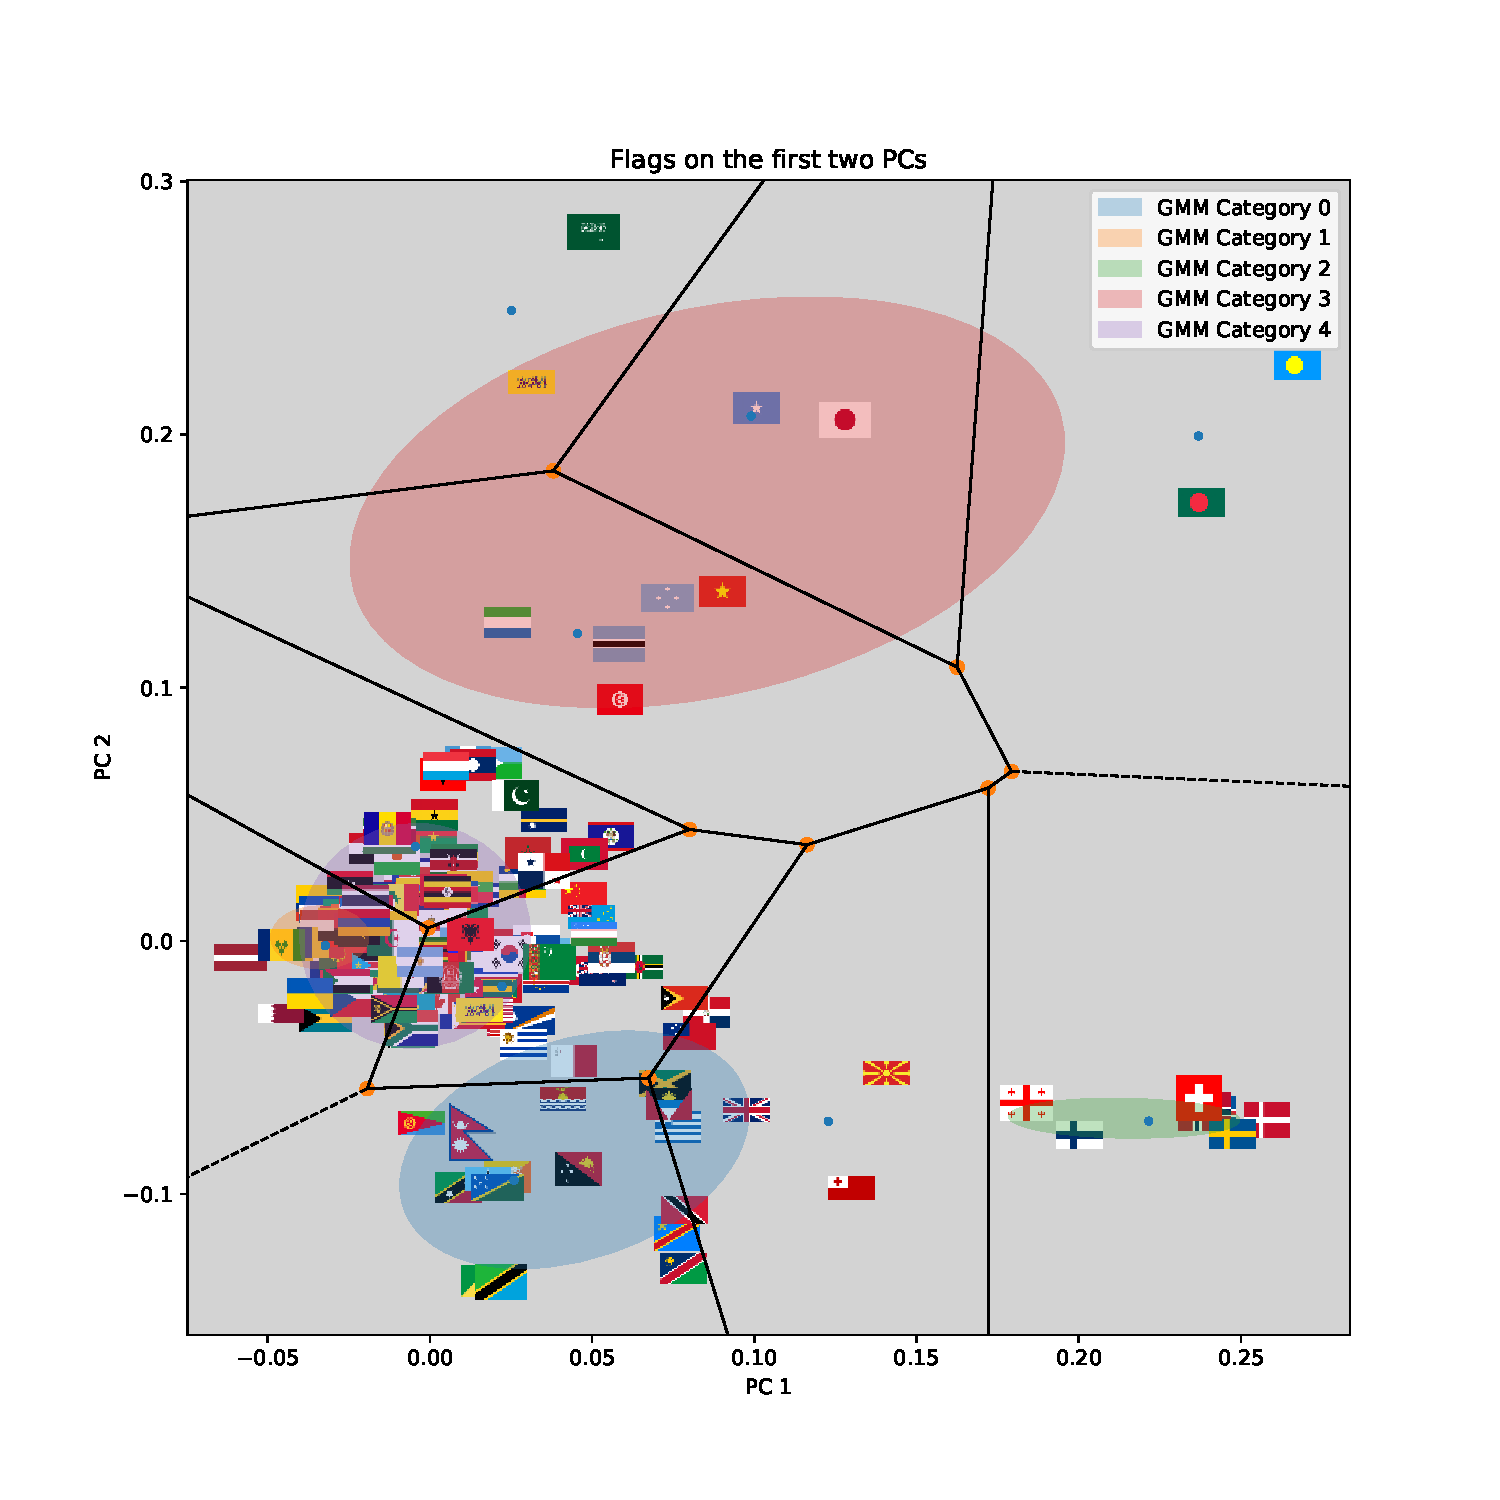
\includegraphics[width=0.8\textwidth]{./res/flags-kmeans-gmm.pdf}
    \caption{Flags plotted on the first two principal components of their
    descriptions. A Voronoi diagram with the boundaries of \(10\)-means clusters
    on 2-PCs is overlaid; means are blue points, boundary corners are orange.
    Ellipses are GMM confidence intervals; note that a flag does not have to be
    within an ellipse to be assigned to that category.\label{fig:flag-pca}}
\end{figure}

% \todo{what does each PC mean?}

Unfortunately, many flags are clumped together on the bottom left side and are
hard to differentiate. For one, there are still many PCs that separate these
flags that we are not visualizing that are projected onto just two dimension,
and secondly, many flags are in fact similar! Many of the flags in that large
cluster are either horizontal or vertical tricolors (a flag with three colors,
generally in equally sized bands), and more still are striped.

\subsection*{GMM Clusters}

Category 0 is an interesting Category containing many unique flags. Many in this
category have a diagonal stripe, such as the Solomon Islands, Namibia, and Papua
New Guinea. It contains Nepal, the only non-rectangular flag in the world, and
it contains the flag of the United Kingdom. The Union Jack is inset on the flags
of so many other flags of present or former commonwealth nations, however none
of these flags exist in this category. This could indicate that the Union Jack
is often not a defining feature of those flags; it is possible for a nation to
redefine itself beyond its colonial past.

Category 1 is the largest category at 94 flags, and as such is very
heterogenous, but the large trend is toward tricolors. Samples in this category
include Russia, Azerbaijan, Bulgaria (all tricolors), Antigua and Barbuda, and
Angola (not tricolors).

The GMM also picks up on our observation that the flags with crosses are
isolated in the corner, grouping them all into Category 2. This is the most
homogenous category, consisting exclusively of flags that have a cross in them.

Category 3 grouped together the solid flags with
circles in the middle, but captured a few other flags as well. This category
seems to be flags that are mostly solid colors with a symbol in the middle, like
Vietnam, Tunisia, and Somalia. Of course there are a few outlier tricolors in
Botswana and Sierra Leone.

Finally, Category 4 is the second largest category with eighty flags. Again
there is a wide variety of flags here. Many are common designs and often feature
a symbol in the middle: tricolors (Canada), bicolors (Burkina Faso), and solid
in color (Albania); but as usual it is not without its unique flags like
Wiphala\footnote{A flag representing the native peoples of the Andes, adopted by
Bolivia as one of two national flags.} with its checkerboard pattern, and Bosnia
and Herzegovina with its isosceles triangle in the middle.

We can also examine the similarity between flags in PC space. Calculating the
Euclidean distance between flags, we can get an idea of how distinct a flag is.
Table \ref{tab:similar-flags} lists the four flags with the largest minimum from
every other flag and the four flags nearest other flags. The top four flags are
indeed very distinct, and instantly recognizable. The least distinct flags are
mostly tricolors or other banded designs. Monaco's flag comes in last, which
makes sense because it comprises two horizontal bands of red (on top) and white,
identical to that of Indonesia except in aspect ratio, and a mirror image of
Poland's flag.

\begin{table}[!ht]
    \centering
    \begin{tabular}{clcc}
        \hline
        \textbf{Rank} & \textbf{Flag \& Country} & \textbf{Average Distance} & \textbf{Minimum Distance} \\
        \hline
        1 & Cyprus-Cyprus & 0.664154 & 0.588152 \\
        2 & Wiphala-Bolivia & 0.642601 & 0.577935 \\
        3 & Saint Lucia-Saint Lucia & 0.657576 & 0.565490 \\
        4 & Switzerland-Switzerland & 0.636214 & 0.556419 \\
        % 5 & Kosovo-Kosovo & 0.622579 & 0.543240 \\
        \vdots & \vdots & \vdots & \vdots \\
        % 209 & Paraguay (reverse)-Paraguay & 0.388655 & 0.000000 \\
        210 & Lithuania-Lithuania & 0.303759 & 0.000000 \\
        211 & Ivory Coast-Ivory Coast & 0.363942 & 0.000000 \\
        212 & Mali-Mali & 0.312427 & 0.000000 \\
        213 & Monaco-Monaco & 0.325320 & 0.000000 \\
        \hline
    \end{tabular}
    \caption{Flags ranked by their similarity}
    \label{tab:similar-flags}
\end{table}


\section{Summary and Conclusions}\label{sec:conclusions}

Flags are difficult to categorize, but we can come up with some useful
distinctions. Our models generally grouped flags by prominent shapes and figures
in the design that are easy to describe, as is expected since our features are
extracted from text descriptions of each flag.

Looking back on the tenets of good flag design, many do well: Germanic nations
succeed at being related (rule five), and were placed in the same category by
the GMM. Likewise, Category 3 contains many good flags that only use a few
colors (three), don't contain lettering (four) and keep it simple (one).

More experimentation with alternative dimension reduction methods like \(k\)-SVD
would be interesting. Alternative clustering algorithms could also be fruitful;
it would be interesting to analyze a hierarchical clustering model, so that the
taxonomical nature of flag types is more present: for example, at one level the
taxonomy could distinguish between solid flags and tricolors, and then within
tricolors, further distinction could be made between vertical and horizontal
bands. Finally, instead of analyzing text descriptions, extracting visual
features directly from the flag itself could reveal new patterns not present in
the text.

\section*{Acknowledgements}

The author wishes to thank Maddy Kovaleski for encouraging me to undertake this
flag project for the final project.

\bibliographystyle{abbrv}
\bibliography{HW_References} % make sure this matches the .bib file for your corresponding document. You also have to maintain your references in the .bib file 

% \appendix
% \section*{Appendix A: GMM Categories}
% \begin{table}[h]
%     \centering
%     \begin{tabular}{lllll}
%         \hline
%         \textbf{Category 0} & \textbf{Category 1} & \textbf{Category 2} & \textbf{Category 3} & \textbf{Category 4} \\
%         \hline
%         Afghanistan (Islamic Emirate) & Afghanistan (Islamic Republic) & Albania & Bhutan & Denmark \\
%         Bangladesh & Algeria & Andorra & Democratic Republic of the Congo & Finland \\
%         Botswana & Angola & Argentina & Republic of the Congo & Georgia \\
%         Japan & Antigua and Barbuda & Australia & Dominican Republic & Iceland \\
%         Micronesia & Armenia & State flag of Austria & Greece & Norway \\
%         Palau & Civil flag of Austria & Bahamas & Jamaica & Sweden \\
%         Saudi Arabia & Azerbaijan & Belize & Kiribati & Switzerland \\
%         Sierra Leone & Bahrain & Wiphala & Namibia & \\
%         Somalia & Barbados & Bosnia and Herzegovina & Nepal & \\
%         Tunisia & Belarus & Brazil & North Macedonia & \\
%         Vietnam & Belgium & Brunei & Papua New Guinea & \\
%         & Benin & Burkina Faso & Saint Kitts and Nevis & \\
%         & Civil flag of Bolivia & Burundi & Saint Lucia & \\
%         & State flag of Bolivia & Cambodia & Samoa & \\
%         & Bulgaria & Canada & Solomon Islands & \\
%         & Cameroon & Cape Verde & Tanzania & \\
%         & Chad & Central African Republic & Timor-Leste & \\
%         & Colombia & Chile & Tonga & \\
%         & Comoros & China & Trinidad and Tobago & \\
%         & National flag of Costa Rica & State flag of Costa Rica & United Kingdom & \\
%         & Croatia & Cuba & Taiwan & \\
%         & Cyprus & Czech Republic & & \\
%         & Egypt & Djibouti & & \\
%         & El Salvador & Dominica & & \\
%         & Equatorial Guinea & Ecuador & & \\
%         & Estonia & Eritrea & & \\
%         & France & Eswatini & & \\
%         & Gabon & Ethiopia & & \\
%         & Germany & Fiji & & \\
%         & Guinea & Gambia & & \\
%         & Guinea-Bissau & Ghana & & \\
%         & Haiti & Grenada & & \\
%         & Honduras & Guatemala & & \\
%         & Hungary & Guyana & & \\
%         & India & Iraq & & \\
%         & Indonesia & Israel & & \\
%         & Iran & Kazakhstan & & \\
%         & Ireland & Kenya & & \\
%         & Italy & Kyrgyzstan & & \\
%         & Ivory Coast & Laos & & \\
%         & Jordan & Latvia & & \\
%         & Kuwait & Liberia & & \\
%         & Lebanon & Luxembourg & & \\
%         & Lesotho & Malaysia & & \\
%         & Libya & Maldives & & \\
%         & Liechtenstein & Malta & & \\
%         & Lithuania & Marshall Islands & & \\
%         & Madagascar & Mauritania & & \\
%         & Malawi & Montenegro & & \\
%         & Mali & Morocco & & \\
%         & Mauritius & Myanmar & & \\
%         & Mexico & Nauru & & \\
%         & Moldova & New Zealand & & \\
%         & Monaco & Niger & & \\
%         & Mongolia & North Korea & & \\
%         & Mozambique & Pakistan & & \\
%         & Netherlands & Panama & & \\
%         & Nicaragua & Philippines & & \\
%         & Nigeria & Qatar & & \\
%         & Oman & Serbia & & \\
%         & Palestine & Seychelles & & \\
%         & Paraguay (obverse) & Slovakia & & \\
%         & Paraguay (reverse) & South Africa & & \\
%         & Civil flag of Peru & South Korea & & \\
%         & State flag of Peru & Sri Lanka & & \\
%         & Poland & Suriname & & \\
%         & Portugal & Togo & & \\
%         & Romania & Turkey & & \\
%         & Russia & Turkmenistan & & \\
%         & Rwanda & Tuvalu & & \\
%         & Saint Vincent and the Grenadines & Uganda & & \\
%         & San Marino & Ukraine & & \\
%         & São Tomé and Príncipe & United States & & \\
%         & Senegal & Uruguay & & \\
%         & Singapore & Uzbekistan & & \\
%         & Slovenia & Vanuatu & & \\
%         & South Sudan & Abkhazia & & \\
%         & Spain & Kosovo & & \\
%         & Sudan & Northern Cyprus & & \\
%         & Syria (revolution) & Somaliland & & \\
%         & Syria (Ba'athist) & & & \\
%         & Tajikistan & & & \\
%         & Thailand & & & \\
%         & United Arab Emirates & & & \\
%         & Vatican City & & & \\
%         & Civil flag of Venezuela & & & \\
%         & State flag of Venezuela & & & \\
%         & Yemen & & & \\
%         & Zambia & & & \\
%         & Zimbabwe & & & \\
%         & Sahrawi Arab Democratic Republic & & & \\
%         & South Ossetia & & & \\
%         & Transnistria & & & \\
%         & Russia & & & \\
%         \hline
%     \end{tabular}
%     \caption{Add caption here}
%     \label{tab:flags_table}
% \end{table}


\end{document}
